\documentclass[border=12pt]{standalone}
\usepackage[T1]{fontenc}
\usepackage{helvet}
\renewcommand{\familydefault}{\sfdefault}
\usepackage{amsmath}
\usepackage{tikz}
\usetikzlibrary{positioning,arrows.meta,calc,fit,backgrounds,shapes.geometric,shapes.misc}

% palette
\definecolor{spinefill}{RGB}{232,234,238}
\definecolor{spinedraw}{RGB}{110,118,130}
\definecolor{liverfill}{RGB}{246,247,249}
\definecolor{liverdraw}{RGB}{168,175,184}
\definecolor{teald}{RGB}{13,110,122}
\definecolor{tealfill}{RGB}{223,239,240}
\definecolor{amber}{RGB}{193,118,18}
\definecolor{amberfill}{RGB}{250,240,222}
\definecolor{inkc}{RGB}{33,38,46}
\definecolor{salmon}{RGB}{193,110,95}
\definecolor{salmonfill}{RGB}{244,225,220}

% badges
\newcommand{\bnew}{\colorbox{teald}{\textcolor{white}{\scriptsize\bfseries NEW}}\hspace{2pt}}
\newcommand{\bchg}{\colorbox{amber}{\textcolor{white}{\scriptsize\bfseries CHANGED}}\hspace{2pt}}

\begin{document}
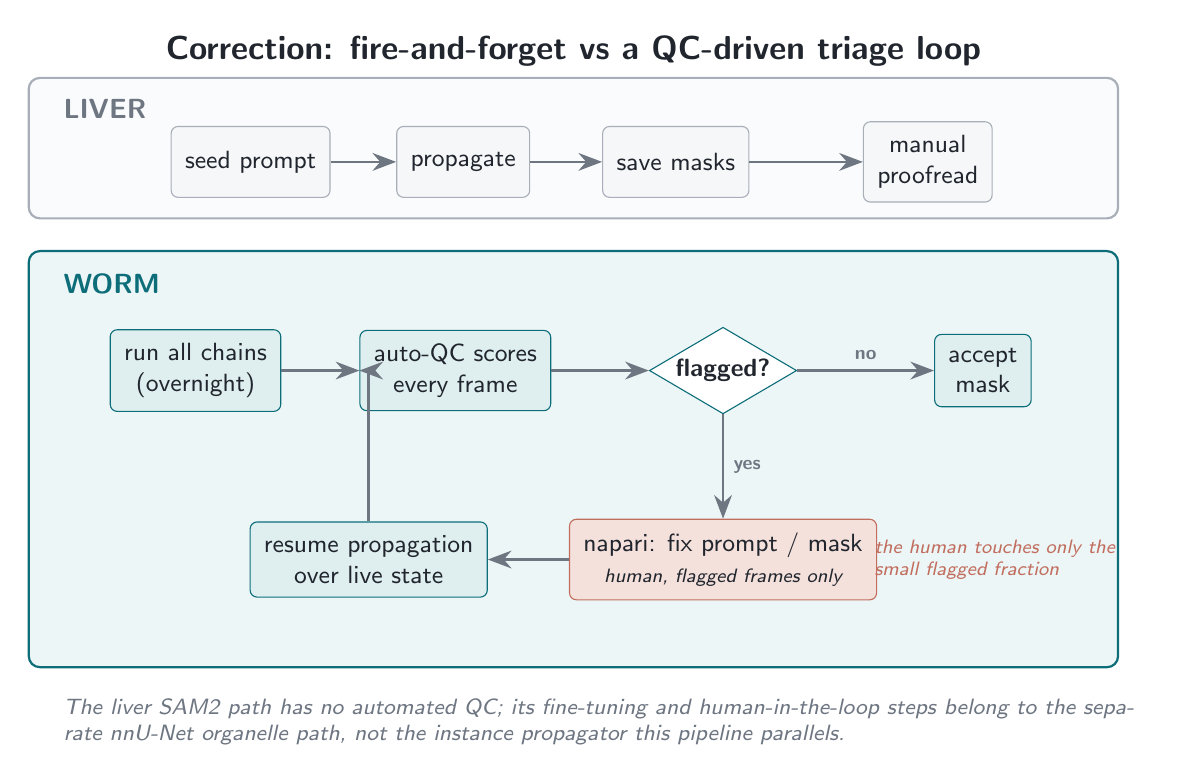
\begin{tikzpicture}[
  band/.style={rounded corners=4pt, line width=0.8pt},
  lbl/.style={font=\bfseries},
  lproc/.style={rounded corners=2.5pt, draw=liverdraw, fill=liverfill, text=inkc, font=\small, align=center, inner sep=5pt, minimum height=0.9cm},
  wproc/.style={rounded corners=2.5pt, draw=teald, fill=tealfill, text=inkc, font=\small, align=center, inner sep=5pt, minimum height=0.9cm},
  dec/.style={diamond, aspect=1.7, draw=teald, fill=white, text=inkc, font=\small\bfseries, inner sep=1pt},
  arr/.style={-{Stealth[length=3mm]}, line width=1.0pt, spinedraw},
  elbl/.style={font=\scriptsize\bfseries, text=spinedraw},
]

\node[align=center, font=\large\bfseries, text=inkc] at (0.4,3.35)
  {Correction: fire-and-forget vs a QC-driven triage loop};

% ============ LIVER (linear) ============
\node[band, draw=liverdraw, fill=liverfill!55, fit={(-6.4,1.35)(7.2,2.9)}] {};
\node[lbl, text=spinedraw, anchor=west] at (-6.2,2.62) {LIVER};
\node[lproc] (lp1) at (-3.7,1.95) {seed prompt};
\node[lproc] (lp2) at (-1.0,1.95) {propagate};
\node[lproc] (lp3) at (1.7,1.95) {save masks};
\node[lproc] (lp4) at (4.9,1.95) {manual\\proofread};
\draw[arr] (lp1)--(lp2); \draw[arr] (lp2)--(lp3); \draw[arr] (lp3)--(lp4);

% ============ WORM (loop) ============
\node[band, draw=teald, fill=tealfill!55, fit={(-6.4,-4.35)(7.2,0.7)}] {};
\node[lbl, text=teald, anchor=west] at (-6.2,0.4) {WORM};

\node[wproc] (run)  at (-4.4,-0.7) {run all chains\\(overnight)};
\node[wproc] (qc)   at (-1.1,-0.7) {auto-QC scores\\every frame};
\node[dec]   (flag) at (2.3,-0.7)  {flagged?};
\node[wproc] (acc)  at (5.6,-0.7)  {accept\\mask};
\node[wproc, draw=salmon, fill=salmonfill] (fix) at (2.3,-3.1) {napari: fix prompt / mask\\{\scriptsize\itshape human, flagged frames only}};
\node[wproc] (res)  at (-2.2,-3.1) {resume propagation\\over live state};

\draw[arr] (run)--(qc);
\draw[arr] (qc)--(flag);
\draw[arr] (flag)--node[elbl,above]{no}(acc);
\draw[arr] (flag)--node[elbl,right]{yes}(fix);
\draw[arr] (fix)--(res);
\draw[arr] (res) |- (qc);

% human-only note
\node[align=left, font=\scriptsize\itshape, text=salmon, text width=3.4cm, anchor=west] at (4.1,-3.1)
  {the human touches only the small flagged fraction};

% ============ footnote ============
\node[align=left, font=\footnotesize\itshape, text=spinedraw, text width=13.6cm, anchor=north west] at (-6.2,-4.75)
  {The liver SAM2 path has no automated QC; its fine-tuning and human-in-the-loop steps belong to the
   separate nnU-Net organelle path, not the instance propagator this pipeline parallels.};
\end{tikzpicture}
\end{document}
